%% $RCSfile: proj_proposal.tex,v $
%% $Revision: 1.4 $
%% $Date: 2017/10/06 02:55:50 $
%% $Author: kevin $

\documentclass[11pt, a4paper, twoside, openright]{report}

\usepackage{float} % lets you have non-floating floats

\usepackage{url} % for typesetting urls
\usepackage{hyperref}
\usepackage[final]{pdfpages}

%  We don't want figures to float so we define
%
\newfloat{fig}{thp}{lof}[chapter]
\floatname{fig}{Figure}

%% These are standard LaTeX definitions for the document
%%
\title{Proposal - aWall: Collaboration Support for Retrospectives}
\author{Simon Glew}

%% This file can be used for creating a wide range of reports
%%  across various Schools
%%
%% Set up some things, mostly for the front page, for your specific document
%
% Current options are:
% [ecs|msor|sms]          Which school you are in.
%                         (msor option retained for reproducing old data)
% [bschonscomp|mcompsci]  Which degree you are doing
%                          You can also specify any other degree by name
%                          (see below)
% [font|image]            Use a font or an image for the VUW logo
%                          The font option will only work on ECS systems
%
\usepackage[image,ecs,behons]{vuwproject} 

% You should specifiy your supervisor here with
%     \supervisor{Firstname Lastname}
% use \supervisors if there are more than one supervisor
\supervisor {Dr. Craig Anslow}
% Unless you've used the bschonscomp or mcompsci
%  options above use
%   \otherdegree{OTHER DEGREE OR DIPLOMA NAME}
% here to specify degree

% Comment this out if you want the date printed.
\date{}

\begin{document}

% Make the page numbering roman, until after the contents, etc.
\frontmatter

%%%%%%%%%%%%%%%%%%%%%%%%%%%%%%%%%%%%%%%%%%%%%%%%%%%%%%%

\begin{abstract}
Agile does not have a online tool that allows integration to online tools and allows users to use this integration with agile retrospectives. 
This is a problem as it means either product teams have to either be co-located or have to be all parts of agile meetings using a third party meeting tool such as Skype. 
Integrating an agile retrospective method within aWall will allow users to do all agile meetings within one online agile tool.  

\end{abstract}

%%%%%%%%%%%%%%%%%%%%%%%%%%%%%%%%%%%%%%%%%%%%%%%%%%%%%%%

\maketitle

%\tableofcontents

% we want a list of the figures we defined
%\listof{fig}{Figures}

%%%%%%%%%%%%%%%%%%%%%%%%%%%%%%%%%%%%%%%%%%%%%%%%%%%%%%%

\mainmatter

%%%%%%%%%%%%%%%%%%%%%%%%%%%%%%%%%%%%%%%%%%%%%%%%%%%%%%%

\section*{Introduction} 

aWall is a tool used to facilitate agile meetings using touch screens within software teams that helps them to have access to information in a single located place that everyone can access, unlike tools such as physical cardwalls. aWall is a project that is based in Switzerland at FHNW that was built by Professor Martin Kropp and Dr. Craig Anslow. The current aWall project progress can be found here: \url{https://www.youtube.com/watch?v=fzCnjnpRiTI}

\begin{figure}[h]
\centering
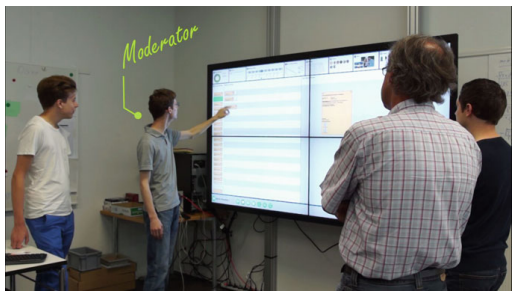
\includegraphics{aWall_introduction}
\caption{Project aWall - digital agile cardwall being used}
\end{figure}

This project is working on the retrospective part of the agile methodology to find and implement a solution that can be integrated within the current system that has already been built.  

\section*{Background}
Retrospectives are meetings held within agile teams, involving all members of the team and is held at the end and just after an iteration of work \cite{AgileRetrospectivesEstherDerby,GettingValueFromRetrospectives}. The retrospective is used for not only celebrating the success of work from the last retrospective, but also the failures and lessons that can be learnt from them \cite {normanKeith}. The retrospective is normally facilitated by a third party member who does not have a personal stake in the in the content or outcome of the meeting, therefore being able to remain neutral during the meeting \cite{normanKeith,retrospectiveFacilator}. Retrospectives are used to reflect on the work done since the last retrospective and the problems that the team faced within this work. \cite{AgileRetrospectivesEstherDerby}. aWall is a online tool that allows for collaboration within a team when it comes to agile practices \cite{xp2017_aWall}, including the aqile practice of retrospectives. With the tool being online, it allows teams to seperate members while still all members can include thoughts and feelings to the agile practices within the team.  

\section*{The Problem}

The problem that this project is attempting to solve is attempting to find a solution to help facilitate agile retrospectives that can support differently located members within a software team. This is a problem as this puts a major restriction on software teams to attempt to co-locate their different software teams, as there isn’t one tool that allows sprint retrospectives for differently located teams. 

This will be achieved by creating a solution to facilitate different forms of agile retrospectives within the aWall product, by researching, implementing and evaluating the different solutions by user testing.

\section*{Proposed Solution}
During this project, I would like to implement 4 different retrospective methods within the aWall project, with of them being implemented in the first four implementations.

The four methods that have been chosen are: 

\begin{itemize}
\item The 3W's method/Mad, Sad and Glad. \\
This method has been chosen due to my experience with it in both academic and industry use, this will be the first method to be implemented, during the first iteration of work. This method will be based off the method outlined within the Ester Derby book \cite{AgileRetrospectivesEstherDerby}.
\end{itemize}
\noindent
The next three methods have been chosen using the methods outlined within the Ester Derby and Norman Keith books \cite{AgileRetrospectivesEstherDerby, normanKeith}.

\begin{itemize}
\item Timeline (5.1)
\item Brainstorming/Filtering (6.1)
\item Short Subjects (7.4)
\end{itemize}

All methods will be using the same activities to set the stage and conclude the retrospective, these are:
\begin{itemize}
\item \textbf{Setting the stage:} Check-in (4.1)
\item \textbf{Conclusion:} +/Delta (8.1)
\end{itemize}

\noindent
The Proposed time line for this project can be found below: \\

\noindent
\textbf{Iteration One:}  6th April - 20th April

\begin{itemize}
\item Familiarization of the aWall codebase
\item Finish Project Proposal
\item Researching and Picking of the other 3 retrospective methods
\item Agile Retrospective Method: 3W's
	\begin{itemize}
		\item Planning
        \item Implementation
        \item Testing
	\end{itemize}
\end{itemize}

\noindent
\textbf{Iteration Two:}  20th April - 4th May

\begin{itemize}
\item Readings around Agile Retrospectives for background section of report
\item Ethics Application (Due: 30th April)
\item Agile Retrospective Method: Timeline
	\begin{itemize}
		\item Planning
        \item Implementation
        \item Testing
	\end{itemize}
\end{itemize}

\noindent
\textbf{Iteration Three:}  4th May - 18th May

\begin{itemize}
\item Readings around Agile Retrospectives for background section of report
\item Agile Retrospective Method: Brainstorming/Filtering
	\begin{itemize}
		\item Planning
        \item Implementation
        \item Testing
	\end{itemize}
\end{itemize}

\noindent
\textbf{Iteration Four:}  18th May - 1st June

\begin{itemize}
\item Readings around Agile Retrospectives for background section of report
\item Agile Retrospective Method: Short Subjects
	\begin{itemize}
		\item Planning
        \item Implementation
        \item Testing
	\end{itemize}
\end{itemize}

\noindent
\textbf{Iteration Five:}  1st June - 8th June

\begin{itemize}
\item Progress Report \\
\end{itemize}

A plan for the second trimester of work will be finalized before the end of the final iteration (8th June). A rough outline plan can been seen below:
\begin{itemize}
\item \textbf{August:} User testing of different retrospectives.
\item \textbf{September:} Implement the most effective method of retrospective into the aWall project and analysis of user testing.
\item \textbf{October:} Writing of the final report.
\end{itemize}

Using the implementation of the four-different agile retrospective methods and the results from the user testing of the different methods, I should be able to implement the most effective retrospective method into the aWall project. All four retrospective methods that are going to be implemented will be done using the same technologies that the current aWall project uses, using jQuery as the frontend framework, due to this first stage not being integrated within aWall, there will be no backend to this project, with all required saving of information being done within the browsers memory. \\

The final solution that will be integrated within the aWall project will be using the full design and libraries of the current aWall project, this solution will also be integrated with the backend that is currently setup within the project to do the saving of the data instead of it being held within the browsers memory. This solution will override the current retrospective section of the aWall codebase.

\section*{Evaluating your Solution}

The first part of evaluating the solution that is created is to do user testing on the four different retrospective methods, this will involve taking users through a agile retrospective using one of the four methods within the tool that is created. For this project, I will be attempting to user test on current third year engineering students within Victoria University currently taking the Engineering project courses (ENGR301 - 302). The tasks that I will get the users to perform will be based on what retrospective method is chosen as each method will need to have its own unique tasks to complete. Once the tasks have been completed, questions will be asked of the students of how they felt about using the specific retrospective method, these questions can be found in the ethics section below. Each team should hopefully participate within two different retrospectives using two different methods that were created. \\

Using the data gained from the user study, I will be able to make a decision on what parts of the retrospectives worked well and what didn't when used by users. From this decision, I will be able to craft a retrospective activity to go within the aWall codebase that uses the best parts that were found from the user study. 

\section*{Resource Requirements}

\subsection*{Ethics} \label{ethics}

Ethics approval will be needed for user testing in the second trimester of the year, the deadline for getting it is the during iteration two (30th April). 

\textbf{Ethics needs more details. Start filling out the forms and attach them with your proposal. This should include a consent form and the kinds of questions you will be asking during the study.}

\subsection*{Safety}

There are no safety concerns during the projects lifecycle.

\subsection*{Budget}

Specialized equipment is required for this project. A large screen, touch overlay for the screen and a computer to run the device and aWall project will be required. Approximate value around \$10,000. The quotes for the required equipment can be seen in the appendix.

\subsection*{Space and Access}

The codebase for this project will be found on both the Victoria University Gitlab \url{https://gitlab.ecs.vuw.ac.nz/} and the FHNW Gitlab \url{https://gitlab.fhnw.ch}. The Gitlab for ecs will be the main source of management for the project with the issue tracker and wiki being used for the project.

This project will also require a room to house and demonstrate on the large touch screen. This room will also be used for conducting the user studies in the second Trimester, a date for this study will be confirmed at a later date.

\subsection*{Intellectual Property}

All intellectual property for this project will be property of their respective parties

% %%%%%%%%%%%%%%%%%%%%%%%%%%%%%%%%%%%%%%%%%%%%%%%%%%%%%%%
% \backmatter
% %%%%%%%%%%%%%%%%%%%%%%%%%%%%%%%%%%%%%%%%%%%%%%%%%%%%%%%

\nocite{xp2017_aWall, sourceVis2013, SourceVis2010, DBLP:conf/agiledc/GossageBB15, code-space-combining-touch-devices-and-skeletal-tracking-to-support-developer-meetings, craigBook, DBLP:conf/agiledc/GhanamWM08}

\bibliographystyle{acm}
\bibliography{biblography}


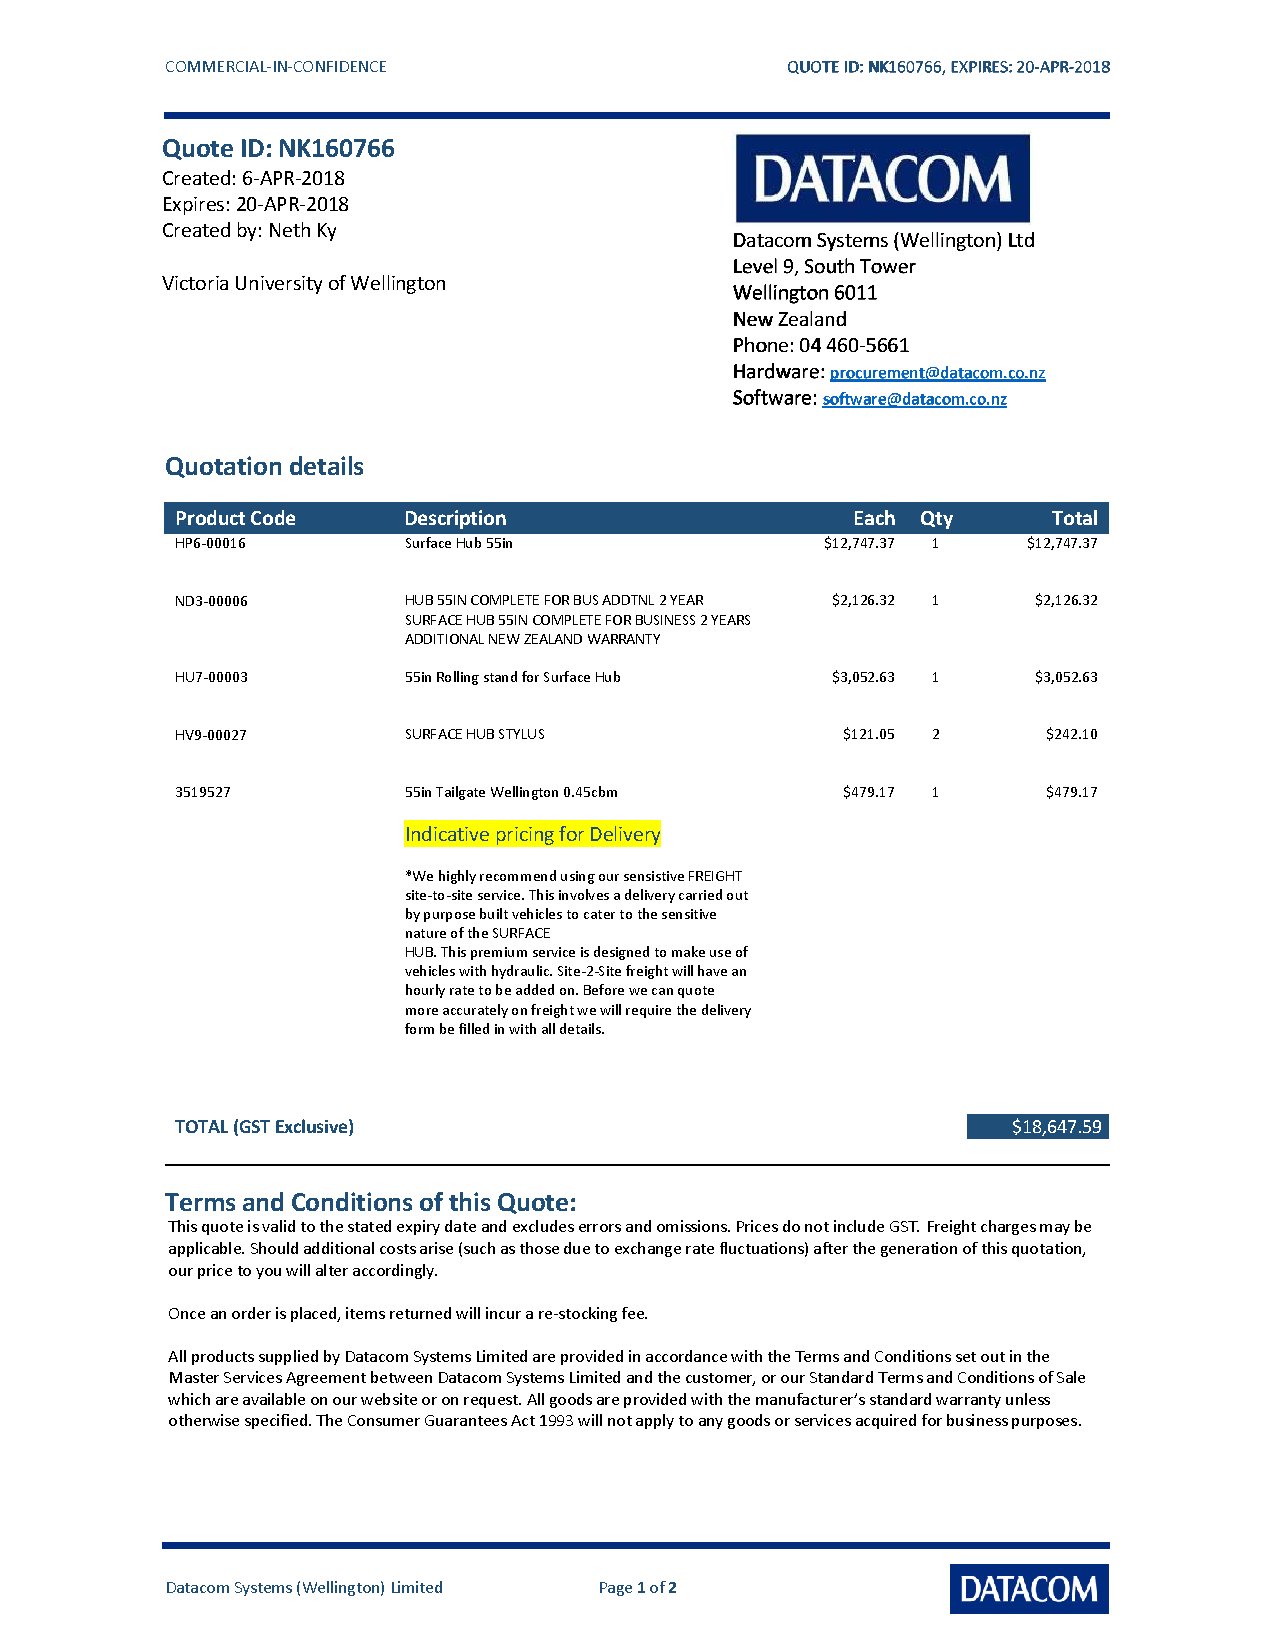
\includepdf[pages=-]{SurfaceHubQuote.pdf}
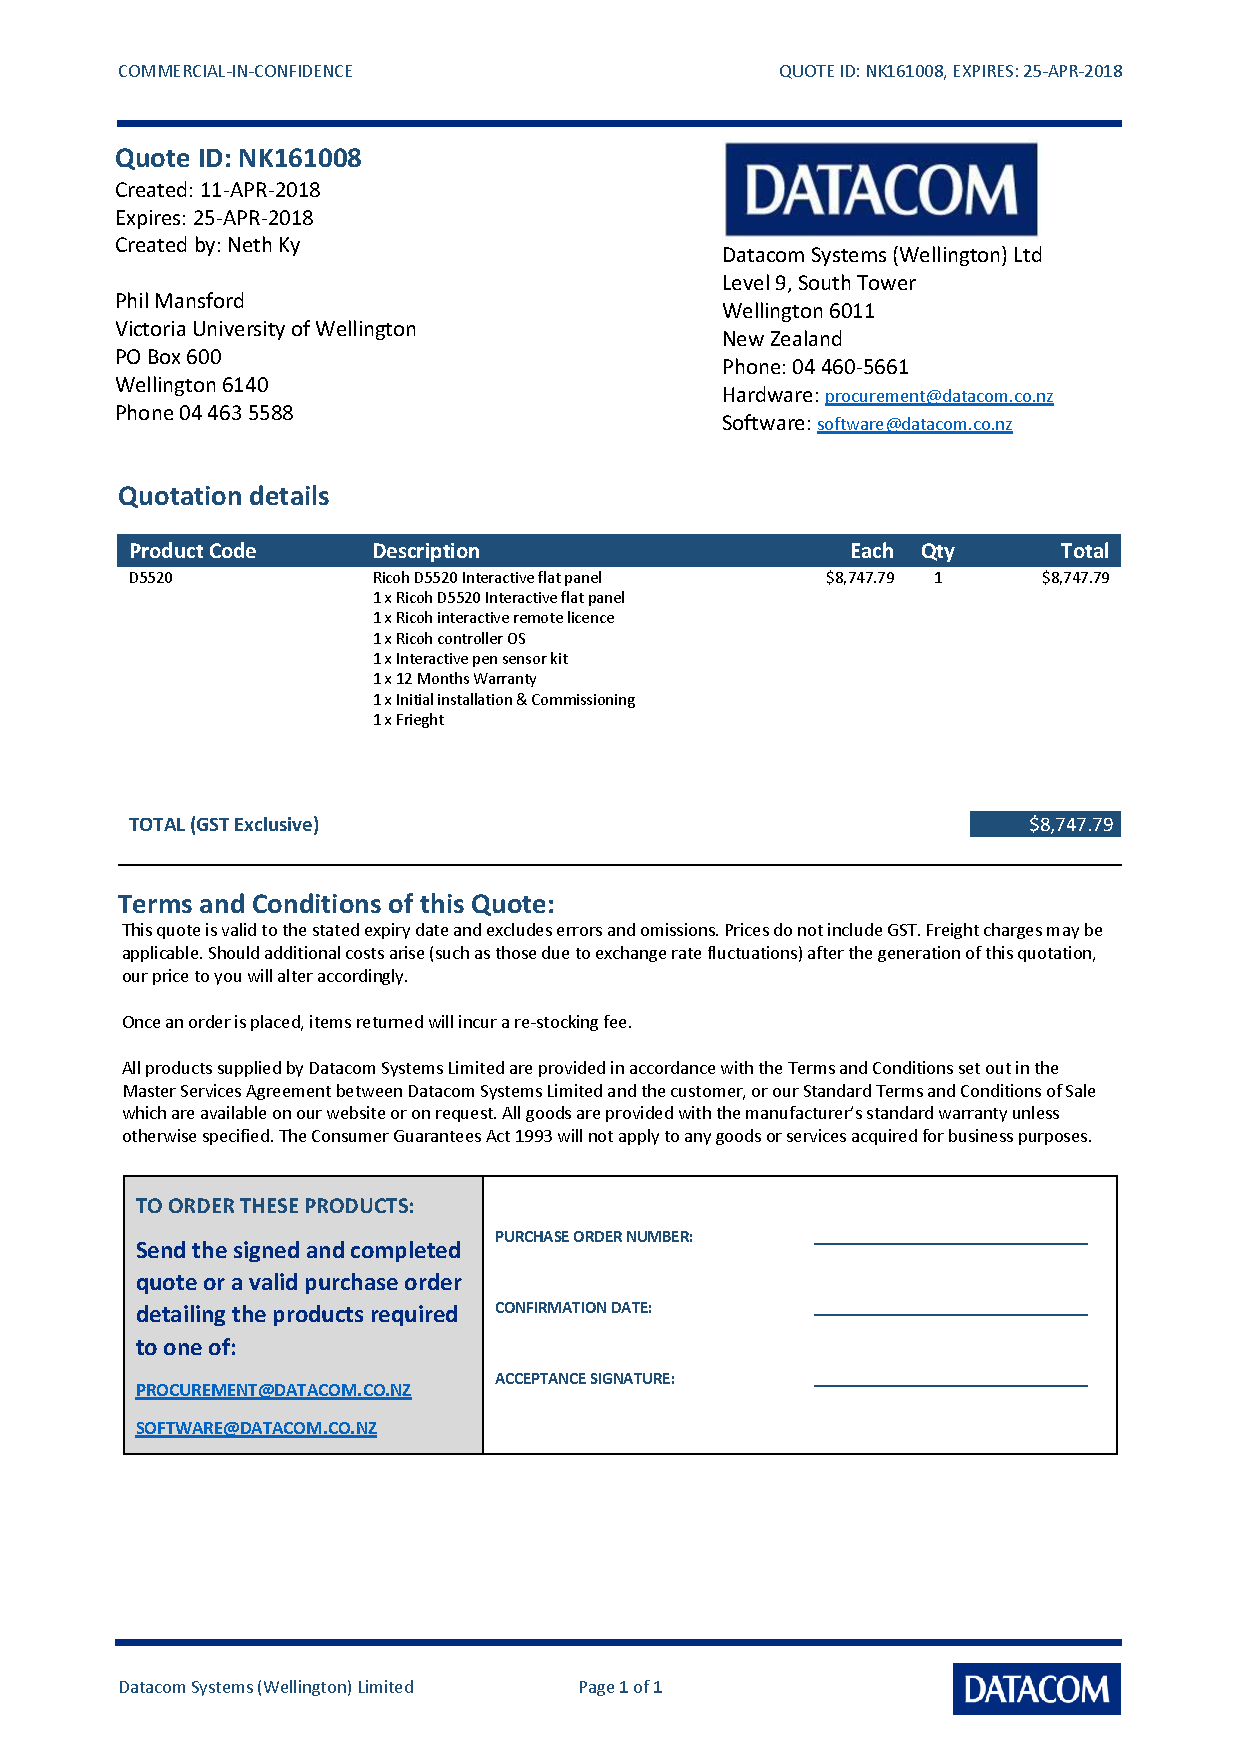
\includepdf[pages=-]{Victoria_University_of_Wellington_-_NK161008.pdf}
\end{document}
